\chapter{\babSatu}
\section{Masuk ke sistem}
Para pengelola pertama kali akan mendapatkan surat elektronik yang berisi informasi akun dan sandi untuk masuk ke aplikasi ini. Selain itu, disertakan juga tautan untuk masuk ke aplikasi untuk mengelola penilaian diri secara \textit{online}. Ilustrasinya ditunjukkan pada \figurename~\ref{fig:email4admin}.
\begin{figure}[h]
  \begin{center}
    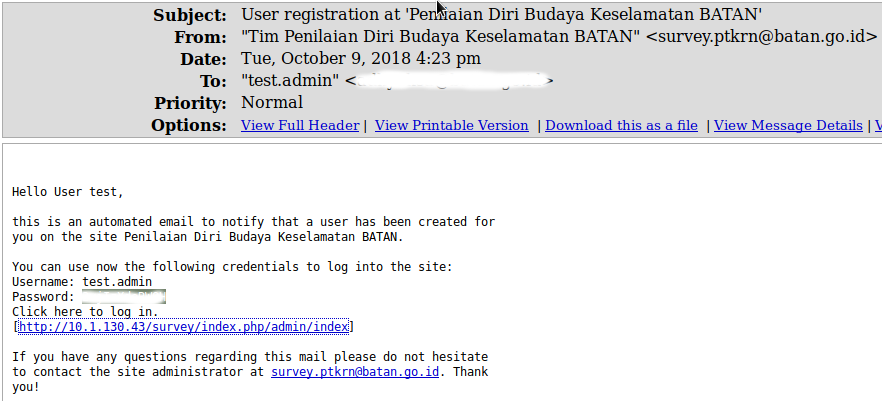
\includegraphics[scale=.35]{pics/surat4admin.png}
    \caption{Surat elektronik pagi pengelola di setiap satker}
    \label{fig:email4admin}
  \end{center}
\end{figure}

Jika pengelola masuk ke aplikasi melalui tautan yang diberikan melalui surat elektronik seperti ditunjukkan di \figurename~\ref{fig:email4admin}, pengelola akan menjumpai dialog seperti \figurename~\ref{fig:login} melalui peramban internetnya.
\begin{figure}
  \begin{center}
    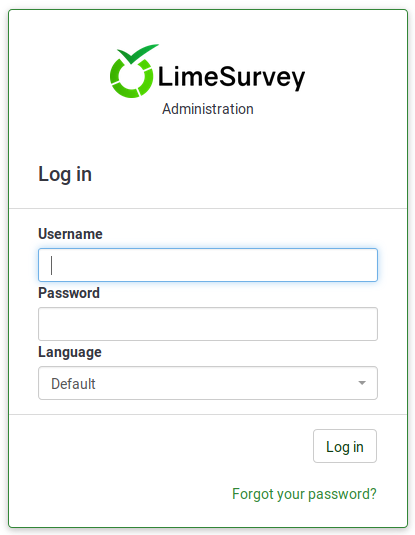
\includegraphics[scale=.45]{pics/login.png}
    \caption{Dialog \textit{login}}
    \label{fig:login}
  \end{center}
\end{figure}

Selanjutnya, pengelola akan masuk ke sistem seperti ditunjukkan \figurename~\ref{fig:masukPertama}.
\begin{figure}
  \begin{center}
    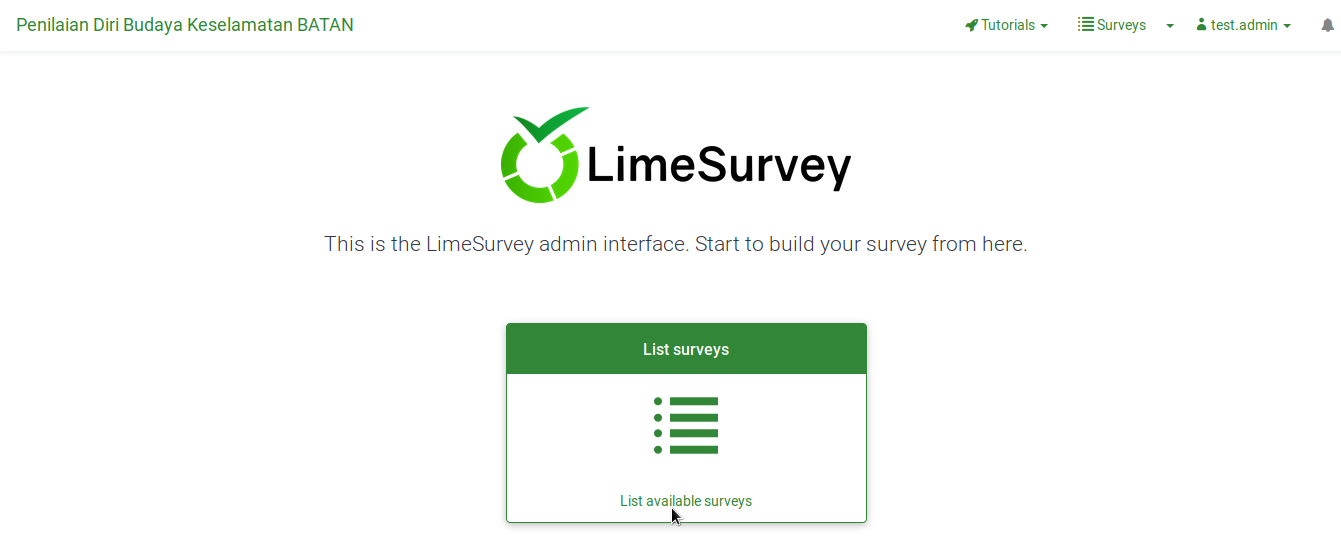
\includegraphics[scale=.35]{pics/masukPertama.png}
    \caption{Halaman pertama yang akan dijumpai saat pertama kali masuk ke sistem}
    \label{fig:masukPertama}
  \end{center}
\end{figure}

\section{Memperbarui sandi}
Ketika, karena satu dan lain hal, pengelola lupa terhadap sandi akunnya, pengelola dapat meminta aplikasi untuk memperbarui sandi. Hal ini dapat dilakukan dengan melakukan klik pada menu ''Forgot your password?'' seperti terlihat di \figurename~\ref{fig:login}. Selanjutnya, pengguna akan menjumpai dialog seperti ditunjukkan pada \figurename~\ref{fig:recoverySandi}. Pengelola memerlukan informasi tentang nama lengkapnya serta alamat surat elektroniknya.

\begin{figure}
  \begin{center}
    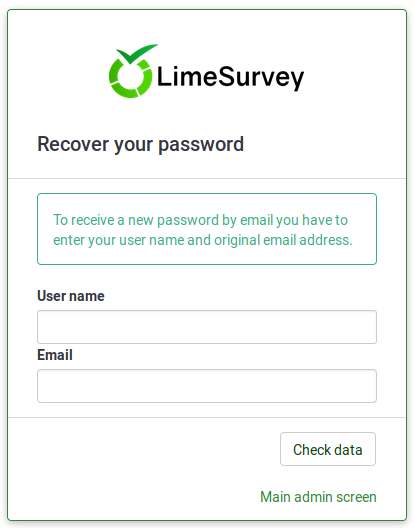
\includegraphics[scale=.35]{pics/recoverPasswd.png}
    \caption{Dialog untuk memperbarui sandi}
    \label{fig:recoverySandi}
  \end{center}
\end{figure}

Setelah pengelola memasukkan informasi yang diperlukan, aplikasi akan mengeluarkan dialog konfirmasi seperti ditunjukkan \figurename~\ref{fig:konfirmasiSandi}.
\begin{figure}
  \begin{center}
    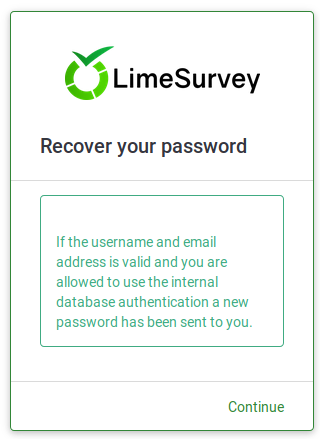
\includegraphics[scale=.35]{pics/recoverPasswd1.png}
    \caption{Dialog konfirmasi untuk memperbarui sandi}
    \label{fig:konfirmasiSandi}
  \end{center}
\end{figure}
